\documentclass[a4paper,12pt,twoside]{report}

%%% PACKAGES %%%


\usepackage{polyglossia}
\setdefaultlanguage[variant=uk]{english} % change to your language
%\setotherlanguage{czech} % if you need a specific part written in another language

% hyphenation rules for specialized words

%\AtBeginDocument{
%\hyphenation{pho-ton quan-tum}
%}

\usepackage{fontspec}

\usepackage[english=british]{csquotes}
\usepackage[xetex]{graphicx}

% see biblatex documentation
\usepackage[sorting=none,style=phys,backend=biber,defernumbers=true]{biblatex}
\usepackage[unicode]{hyperref}
\usepackage{xcolor}
\usepackage{amsmath}
\usepackage[font=small,labelfont=bf]{caption}
\usepackage{fancyhdr}
\usepackage{titlesec}
\usepackage{pdfpages}
\usepackage{microtype}
\usepackage{unicode-math}

% needed for a specific command changing bibliography formatting
\usepackage{xpatch}

% Libertinus fonts
\usepackage{libertinus-otf}


\usepackage{comment}
\usepackage{marginnote}
\usepackage{sidenotes}

\usepackage{lastpage}

% Custom command to create margin notes with author, color, and text size
\newcommand{\alenote}[1]{%
    \sidenote{\tiny \textcolor{green}{\textbf{Alessio:}} #1}%
}

% Custom command to create margin notes with author, color, and text size
\newcommand{\profnote}[1]{%
    \sidenote{\tiny \textcolor{red}{\textbf{Prof:}} #1}%
}


% At the moment, STIX looks better than Libertinus Math, but that will hopefully change soon.
% feel free to comment this out and try Libertinus Math
\setmathfont{STIX2Math.otf}

% metadata for the PDF file
\hypersetup{
pdfauthor={Alessio Martini},
pdftitle={The Title of the Thesis},
pdfsubject={Physics},
pdfkeywords={symmetries, anomalies, quantum mechanics}
}



%%% BIBLIOGRAPHY %%%

\addbibresource{bibliography.bib}


% you may put the publications you authored in a separate category
\DeclareBibliographyCategory{MyArticles}
\addtocategory{MyArticles}{EssinGriffiths:10.1119/1.2165248}
\addtocategory{MyArticles}{Bonneau_2001}


% force the order you want by referencing them all here using \nocite

\nocite{EssinGriffiths:10.1119/1.2165248}
\nocite{Bonneau_2001}
 
\nocite{landau1991quantum} 
\nocite{garfken67:math}
\nocite{gradshteyn2007}

\nocite{Holstein:10.1119/1.4867052}
\nocite{Jackiw:216395}
\nocite{Coon_2002}

%%% BIBLATEX OPTIONS AND TWEAKS %%%

% Biblatex enables editing .bib entries and configuring everything in your LaTeX document

% get rid of the months
\DeclareSourcemap{
  \maps[datatype=bibtex]{
    \map[overwrite]{
      \step[fieldset=month, null]
    }
  }
}


% declare special bibliography contexts with optional prefixes
\DeclareRefcontext{myarticles}{labelprefix=A}
\DeclareRefcontext{books}{labelprefix=B}

% change the typesetting of reference numbers in the bibliography

\DeclareFieldFormat{labelnumberwidth}{#1\hspace{10pt}}

% declare command \citenum that prints a plain reference number
% can be used in a sentence

\DeclareCiteCommand{\citenum}
  {\printtext[bibhyperref]{\printfield{labelprefix}}}
  {\printtext[bibhyperref]{\printfield{labelnumber}}}
  {}
  {}


% produce clickable URL links for theses
\letbibmacro{ORIG-institution+location+date}{institution+location+date}
\renewbibmacro*{institution+location+date}
{\iffieldundef{url}
		{\usebibmacro{ORIG-institution+location+date}}
		{\href{\thefield{url}}{\usebibmacro{ORIG-institution+location+date}}}
}

% small caps typesetting of author names
\DeclareNameWrapperFormat{author}{\textsc{#1}}

% make the 'and' between the last two authors upright and not small caps
% taken from biblatex.def and modified
\DeclareDelimFormat{finalnamedelim}{
\textup{
  \ifnumgreater{\value{liststop}}{2}{\finalandcomma}{}%
  \addspace\bibstring{and}\space
  }
}


% after the authors list, there is a colon and a newline
\renewcommand{\labelnamepunct}{\addcolon\newline}

% the newline between name and journal is tricky to add, because there is no command to redefine.
% here is some black magic using the package xpatch
% taken from https://tex.stackexchange.com/questions/351397/biblatex-add-line-breaks-after-author-and-title
\makeatletter
\def\do#1{
  \ifcsdef{blx@bbx@#1}
    {\xpatchbibdriver{#1}
       {\printlist{language}%
        \newunit\newblock}
       {\printlist{language}%
        \printunit{\addcomma\newline}}
       {}{}}
    {}}
\abx@doentrytypes{}
\makeatother


% make the font size smaller for bibliography
\renewcommand*{\bibfont}{\footnotesize}
 

% if you don't like titles in quotes, this gets rid of them

%\DeclareFieldFormat[article,inproceedings,patent,incollection]{title}{%
%  \iftoggle{bbx:chaptertitle}
%    {#1\isdot}
%    {}%
%}




%%% PAGE HEADERS AND FOOTERS %%%

% !!! the narrow margins are inner margins, while the wider margins are outer margins
% odd-numbered pages  1,3,5,... right side >>> __text____
% even-numbered pages 2,4,6,... left side  >>> ____text__
% see https://en.wikipedia.org/wiki/Canons_of_page_construction

% page layout and margins are left at default settings

\pagestyle{fancy}


% this is here only so LaTeX does not complain
\setlength{\headheight}{15pt}

% the aim here is to have section names in the headings on the inner side
% the way I think this works is:
% when evaluating the \section[shortName]{fullName} command in the text, there is a \sectionmark command inside.
% calling \markboth like below changes the current heading to shortName
% works the same for chapters, both commands are redefined to cover the cases where the chapter does not contain a section immediately
% !!! asterisk commands and table of contents do not contain marks, so you need to do it manually (see the main text)
\renewcommand{\chaptermark}[1]{\markboth{\normalfont\sffamily\textsc{#1}}{}}
\renewcommand{\sectionmark}[1]{\markboth{\normalfont\sffamily\textsc{#1}}{}}

% remove page numbers from the footer and put it into the header (outer side)
\fancyfoot{}
\fancyhf[HLE,HRO]{\thepage}

% redefine plain style to be compatible with fancy (beginning of chapters)
\fancypagestyle{plain}{ %
  \fancyhf{} % remove everything
  \renewcommand{\headrulewidth}{0pt} % remove lines as well
  \renewcommand{\footrulewidth}{0pt}
}


%%% MISCELLANEOUS %%%

% hyperlinks are highlighted using colored text instead of colored boxes
% !!! switch off for printing unless you want the color in print

\hypersetup{
    colorlinks,
    linkcolor=black,
    citecolor=black,
    urlcolor=black
}

% heading styles, sans serif

\def\headingStyle{\sffamily}

\titleformat*{\section}{\LARGE\headingStyle}
\titleformat*{\subsection}{\Large\headingStyle}
\titleformat*{\subsubsection}{\large\headingStyle}
\titleformat{\chapter}[display]
{\huge\headingStyle}{\chaptertitlename\ \thechapter}{20pt}{\Huge\headingStyle}

% in case you like prefixes to distinguish tables and figures from other numbered references

%\renewcommand{\thefigure}{F\arabic{chapter}.\arabic{figure}}
%\renewcommand{\thetable}{T\arabic{chapter}.\arabic{table}}


%%%%%%%%%%%%%%%%%%%%%%%%%%%%%%%%%%%%%%%%%%%%%%%%%%%%%%%%%%%%%%%%%%%%%
\begin{document}

% prima pagina
\newpage
\pagestyle{empty} % empty
\mbox{}
\clearpage

\pagenumbering{roman}

% seconda pagina

\includepdf{title_page.pdf}
\clearpage

% terza pagina
\newpage
%\pagestyle{empty} % empty
\mbox{}
\clearpage

% quarta pagina
\centerline{\headingStyle\Large Abstract}
\bigskip
\noindent
Anomaly refers to a phenomenon where a symmetry, which is present in the classical depiction of a system, becomes disrupted when the system undergoes quantization. In this thesis, we shed light on the instance of scale invariance symmetry breaking during quantization, focusing on the attractive $1/x^2$ potential.

The initial problem presents a significant challenge, as it results in an uncountable and infinite count of bound states, due to its non physical definition. To tackle this issue, we suggest exploring the application of self-adjoint extensions as a possible method to reestablish physically meaningful bound states.
\vfil
{\centering
  \begin{tabular}{rl}
    Title:           & Anomalies in              \\
                     & Quantum Mechanics         \\
    Author:          & Alessio Martini           \\
    Supervisor:      & Noppadol Mekareeya        \\
    Study programme: & Physics                   \\
    Institution:     & Department of Physics,    \\
                     & Faculty of Science,       \\
                     & Milano Bicocca University \\
    Year:            & 2023                      \\
    Pages:           & \pageref{LastPage}
  \end{tabular}
}
\vfil
\noindent
\noindent
This bachelor's thesis, titled \textit{Anomalies in Quantum Mechanics}, is provided for academic purposes. The information and findings presented in this thesis are the result of independent research and should be used as a reference or source of information only.

The author and the academic institution do not guarantee the accuracy, completeness, or up-to-date nature of the information contained in this thesis. 

This thesis is the intellectual property of the author, and any reproduction, distribution, or use for commercial purposes without explicit written permission from the author and the academic institution is prohibited.

The author is solely responsible for the views, opinions, and conclusions presented in this thesis.

The use of any data, equations, or methodologies presented in this thesis for research or practical applications should be done with caution and in accordance with established scientific standards.

Readers are encouraged to consult with professionals or experts in the field for guidance and validation of any information or findings contained herein.
\clearpage

% quinta pagina

\newpage
%\pagestyle{empty} % empty
\mbox{}
\clearpage

% sesta pagina

\mbox{}
\noindent

\vfil
\begin{flushright}
\textit{Ai miei nonni Angelo e Luciana, \\ con infinito affetto.}
\end{flushright}


\vfil
\clearpage

% settima pagina

\pagestyle{fancy}


\chapter*{Preface}
\addcontentsline{toc}{chapter}{Preface}
\markboth{\normalfont\sffamily\textsc{Preface}}{}

This dissertation is primarily based on two papers: the first, authored by Andrew M. Essin and David J. Griffiths, is titled \textit{"Quantum Mechanics of the $1/x^2$ Potential"}~\cite{EssinGriffiths:10.1119/1.2165248}. This paper forms the backbone of the physical aspects discussed in this thesis. The second paper, by G. Bonneau, J. Faraut, and G. Valent, is titled \textit{"Self-Adjoint Extensions of Operators and the Teaching of Quantum Mechanics"}~\cite{Bonneau_2001}. It provides the mathematical methods underpinning the thesis.

\vspace{2mm}
\noindent
This dissertation represents an original, unpublished, and independent work.

\noindent
\parbox{.4\textwidth}{
  Milano
  \\
  November 2023
}
\hfill
\parbox{.4\textwidth}{\flushright{}
  Alessio Martini
  \\
  a.martini25@campus.unimib.it
}

\clearpage

% ottava pagina
\tableofcontents
\markboth{\textsc{Contents}}{}
\clearpage

\newpage
\pagestyle{empty} % empty
\mbox{}
\clearpage

\pagestyle{fancy}
\pagenumbering{arabic}

%%% MAIN TEXT BEGINS %%%
% it is better to have chapters in separate files and include them by \input

\chapter*{Introduction}
\addcontentsline{toc}{chapter}{Introduction}
\markboth{\normalfont\sffamily\textsc{Introduction}}{}
%%%%%%%%%%%%%%%%%%%%%%%%%%%%%%%%%%%%%%%%%

% preamble
This thesis represents an exploration of a connection between the method of self-adjoint extension and the phenomenon of anomalous symmetry breaking referred to scale symmetry in quantum mechanics. At first glance, these two concepts may appear completely independent, but as we delve into the heart of this thesis, you will come to understand the link that binds them in our specific problem.

Through rigorous analysis, critical insights, and a thorough examination of relevant literature, this work strives to elucidate how self-adjoint extensions can shed light on the intricate interplay between symmetries and quantum systems. We aim to provide a bridge between the seemingly abstract world of mathematical operators and the tangible consequences of symmetry breaking in the realm of quantum physics.

By embarking on this intellectual journey, you will gain a deeper appreciation for the profound impact of self-adjoint extensions on the understanding of anomalous symmetry breaking, and how this connection shapes the very foundations of quantum mechanics.

As you embark on the chapters that follow, we invite you to explore this territory of theoretical physics and uncover the relationship between self-adjoint extensions and the anomalies that can emerge when quantum mechanics meets symmetries.

\vspace{4mm}
\noindent
Introducing the contents of the essay we can start saying that it is commonly taught that an attractive potential vanishing at infinity implies a set of bound states that are both discrete and infinite. 
However, we will demonstrate that this holds true only for certain potentials, as discussed in Section~\ref{section:generic_potentials}.

Our discussion will lead us to categorize attractive potentials that vanish at infinity into two groups, and this classification naturally leads to the definition of a special case, namely, the $-\alpha/x^2$ potential. 
This potential exhibits unique characteristics that set it apart from other potentials as we will show in Section~\ref{section:peculiarities}.

We will introduce and employ the method of self-adjoint extension, as described in Section~\ref{section:self_adjoint}, to address the issue that the naive formulation of the special case potential $-\alpha/x^2$ does not result in a Hamiltonian that is an Observable when considered in the context of Quantum Mechanics, as discussed in Section~\ref{section:xsqared_halfaxis}.
Additionally, we will provide a simpler introductory example of the mathematical method: the free particle on the half-axis in Section \ref{section:free_halfaxis}.

At the conclusion of this essay, we will observe that, upon elevating the Hamiltonian operator to the status of an Observable, the scale invariance of our problem has been unexpectedly broken. This anomaly will be examined from two perspectives: the boundary conditions and the bound states.

In conclusion, the essay will establish a connection between the problem discussed and the two-dimensional $\delta$-function potential problem commonly encountered in the literature on anomalies in Quantum Mechanics, as detailed in Section~\ref{section:delta_potential}.

\clearpage

\section*{Classifying symmetry breakings}
In the realm of physics, symmetries are fundamental for unraveling the conservation laws that govern physical systems. However, it is unfortunate that these symmetries can be disrupted.

There are three distinct pathways through which a symmetry, whether continuous or discrete, can be compromised during the investigation of a system. This phenomenon is referred to as "the breaking of a symmetry."

\begin{enumerate}
    \item \textbf{Explicit Symmetry Breaking}:
          \begin{itemize}
              \item \textbf{Description}: Explicit symmetry breaking occurs when external influences or explicitly added terms in a physical system break the symmetry that the system would otherwise possess.
              \item \textbf{Example}: An external magnetic field applied to a material can explicitly break the rotational symmetry of the material's electrons.

                    Or, in a more abstract example, but one that resembles the problem we will discuss: a free particle on the whole real axis obviously possesses parity symmetry and translational symmetry. The introduction of a potential lacking parity unequivocally disrupts both symmetries.
          \end{itemize}

    \item \textbf{Spontaneous Symmetry Breaking}:
          \begin{itemize}
              \item \textbf{Description}: Spontaneous symmetry breaking occurs when the laws governing a physical system are symmetric, \textit{e.g. the Lagrangian}, but the system's ground state (the lowest energy state) does not present the same symmetry.

              \item \textbf{Example}: In a ferromagnetic material \textit{e.g. iron}, the individual magnetic moments of its atoms tend to align in a specific direction. At high temperatures, these magnetic moments are randomly oriented, and the material has no net magnetization. In this state, there is a symmetric orientation of magnetic moments.

                    However, as the temperature decreases, there is a critical temperature called the Curie temperature. Below this temperature, the material spontaneously undergoes a quantum mechanical phase transition, and the magnetic moments align in the same direction, resulting in a net magnetization. The symmetry is spontaneously broken as the material acquires a macroscopic magnetization in a specific direction.

                    This phenomenon is a classic example of spontaneous symmetry breaking in classical physics and is responsible for the behavior of permanent magnets and the Earth's magnetic field.

                    Or, in a more abstract example, but one that resembles the problem we will discuss: a particle in a symmetric double well potential. Even though the system possesses parity symmetry, in Quantum Mechanics, the particle spontaneously chooses one well over the other, breaking the symmetry.
          \end{itemize}

    \item \textbf{Anomalous Symmetry Breaking}:
          \begin{itemize}
              \item \textbf{Description}: Anomalous symmetry breaking is a phenomenon where the process of quantization of a system, \textit{i.e. to solve it using quantum mechanics}, break symmetries that would be preserved in a classical theory.
              \item \textbf{Example}: In quantum field theory, anomalies can result in the violation of classically conserved currents, such as the chiral anomaly in the context of the strong force, which breaks specific symmetries.

                    In our case, the scale invariance of the problems will be broken when the Hamiltonian operator of the problem, originally lacking physical significance, is elevated to the status of a physical Observable.
          \end{itemize}
\end{enumerate}

\noindent
The first two symmetry breaking mechanisms are well known to physicists since the apply to classical as well as quantum systems.
Rather, our discussion will focus on the subject of anomalous symmetry breaking.

Typically, this mechanism is encountered within Quantum Field Theory, such as the chiral anomaly in processes like $\pi^0 \rightarrow 2 \gamma$. However, there are two examples from ordinary quantum mechanics: the two-dimensional $\delta$-potential and the $-1/x^2$ potential. We will study the latter, but as mentioned before, we will establish a connection between them at the end of the essay in Section~\ref{section:delta_potential}, demonstrating that they are not entirely distinct problems.
\cleardoublepage{}

\chapter{Why the \texorpdfstring{$1/x^2$}{inverse squared} potential?} %%%%%%%%%%%%%%%%%%%%%%%%%%%%%%%%%%%%%%%%%

\section{The stationary Schrödinger's Equation}
\label{section:generic_potentials}
In this section, freely inspired by the work of Landau and Lifshitz~\cite{landau1991quantum}, we provide a summary of the analysis of the Schrödinger equation for different cases corresponding to the functional form of a singular potential at the origin. This section aims to justify why we are choosing the particular $-1/x^2$ potential, and further reasons will be discussed during its analysis. 

We consider the time-independent Schrödinger equation which is given as follows:

\begin{equation*}
    \left(- \frac{\hbar^2}{2m}\nabla^2 + V(x) \right) \psi = E \psi
\end{equation*}

\subsection*{General Conditions}
Solutions of the Schrödinger equation must satisfy certain general conditions. The wave function \(\psi(x, t)\) should be continuous throughout all space, even when the potential \(V(x)\) has discontinuities. However, it's essential to note that the continuity of derivatives is not maintained if there exists a surface beyond which the potential energy \(V\) becomes infinite (\(V = \infty\)). In such cases, the wave function \(\psi\) must be zero throughout this region, and the derivatives of \(\psi\) may be discontinuous.

\clearpage

\subsection*{Potential Function}
The potential function \(V(x)\) is assumed to have the form:

\begin{equation*}
    V(x) = -\frac{a}{x^s}, \quad s \in \mathbb{R}, \quad a > 0.
\end{equation*}

\noindent
Let's now analyze what happens for different values of $s$.

\subsubsection{Case: \(s < 0\)}
In this case, the potential is neither singular nor attractive, and there are no issues with the wave function.

\subsection*{Short-Distance Behavior}

For a generic value of \(s\), a wave function that remains finite in a small region (with radius \(r_0\)) around the origin and is zero outside this region leads to uncertainty in the particle's coordinates on the order of \(\hbar/r_0\). The uncertainty in momentum is on the order of \(1/r_0\). The mean values of kinetic and potential energy are given by:

\begin{equation*}
    \langle K \rangle \approx \frac{\hbar^2}{2 m r_0^2} \quad \text{and} \quad \langle V \rangle \approx -\frac{a}{r_0^s}
\end{equation*}

\noindent
This provides an expression for the total energy:

\begin{equation*}
    \langle E \rangle \approx \frac{\hbar^2}{2 m r_0^2} - \frac{a}{r_0^s}
\end{equation*}

\subsubsection{Case: \(s > 2\)}
The total energy becomes arbitrarily negative for sufficiently small \(r_0\), \textit{i.e. \( \langle E \rangle \to -\infty\)}. This implies the existence of stationary states with negative energy levels of arbitrarily large absolute values. The particle's motion in a small region near the origin corresponds to energy levels with large absolute values, and the \textit{ground state} is when the particle is at the origin, resembling a \textit{fall} to \(r = 0\).

\subsubsection{Case: \(s < 2\)}
The energy cannot take arbitrarily large negative values; in fact, \( \langle E \rangle \to +\infty\). The discrete spectrum begins at a finite negative value, indicating that the particle does not fall to the center.

Unlike classical mechanics, where a particle's fall to the center is theoretically possible in any attractive field, quantum mechanics imposes limitations.

\subsection*{Large-Distance Behavior}
The nature of the energy spectrum is influenced by the behavior of the field at large distances. As \(r\) approaches infinity, the negative potential energy tends to zero. For a wave packet \textit{filling} a spherical shell of large radius \(r_0\) and thickness \(\Delta r\), where \(\Delta r\) is much less than \(r_0\), the order of magnitude of kinetic energy is \(\hbar^2/2 m \Delta r^2\), and the one of the potential energy is \(-a/r_0^s\).

This results in the formula for the average energy:

\begin{equation*}
    \langle E \rangle \approx \frac{\hbar^2}{2 m \Delta r^2} - \frac{a}{r_0^s}
\end{equation*}

\noindent
Then, if we consider the limit as $r_0$ approaches infinity and constrain $\Delta r$ to grow proportionally to it, we are led to differentiate again with respect to the values of $s$.

\subsubsection{Case: \(s < 2\)}
The total energy can become negative for sufficiently large \(r_0\), leading to stationary states with negative energy; in fact, \( \langle E \rangle \to 0^-\). This allows the particle to be found at large distances from the origin with a fair probability, implying that there are levels of arbitrarily small negative energy, and the discrete spectrum includes an infinite number of levels, denser toward \(E = 0\).

\subsubsection{Case: \(s > 2\)}
There are no levels of arbitrarily small negative energy; in fact, \( \langle E \rangle \rightarrow 0^+\). The discrete spectrum terminates at a level with a non-zero absolute value, resulting in a finite total number of levels.

%\clearpage

\subsection*{Conclusion}
The analysis of the Schrödinger equation for different values of \(s\) reveals a variety of behaviors. The case \(s = 2\) is a special limit case that separates unstable bound states (\(s > 2\)) from stable ones (\(s < 2\)).

\clearpage

\section{Peculiarities of the \texorpdfstring{$1/x^2$}{inverse squared} potential}
\label{section:peculiarities}
Now that we've understood that the $-1/x^2$ potential could have something different from the other ones, let's investigate some of its peculiarities following the procedure that has been done by Essin and Griffiths~\cite{EssinGriffiths:10.1119/1.2165248}.

First consider the explicit form of the potential we're going to examine:

\begin{equation*}
    V(x) = \begin{cases}
        \infty    & \text{if } x \leq 0 \\
        - a / x^2 & \text{if } x > 0
    \end{cases}
\end{equation*}

which is shown in Figure~\ref{fig:potential}.

\subsection*{The dimensional problem}

Even though we haven't done anything yet, there is already something worth noticing. In fact, from the parameters present in our problem, \textit{i.e. \(\hbar\), \(m\), and \(a\)}, there is no way to construct a quantity with the dimensions of energy.

Let's show it from the dimensional analysis. Our parameters have the following dimension:

\begin{align*}
    [\hbar] = E \cdot T, \quad [m] = E \cdot T^2 \cdot L^{-2}, \quad [a] = E \cdot L^2.
\end{align*}

\noindent
So we want to look for three parameters $\alpha$,$\beta$ and $\delta$ that satisfy

\begin{align*}
    E & = \hbar^\alpha m^\beta a^\delta                                                      \\
      & = (E \cdot T)^\alpha (E \cdot T^2 \cdot L^{-2})^\beta (E \cdot L^2)^\delta           \\
      & = E^{\alpha + \beta + \delta} \cdot T^{\alpha + 2\beta} \cdot L^{-2\beta + 2\delta}.
\end{align*}

\noindent
So we are lead to an equation for each quantity, \textit{i.e. the system}:

\begin{align*}
    \begin{cases}
        E: & 1 = \alpha + \beta + \delta \\
        T: & 0 = \alpha + 2\beta         \\
        L: & 0 = -2\beta + 2\delta
    \end{cases}
    \quad
    \begin{cases}
        1 = - 2\beta + \beta + \beta \\
        \alpha = -2\beta             \\
        \delta = \beta
    \end{cases}
    \quad
    \begin{cases}
        1 = 0            \\
        \alpha = -2\beta \\
        \delta = \beta
    \end{cases}
\end{align*}

\noindent
Se we have no solutions, hence no possible formula for the eigenvalues of the Hamiltonian.
The issue will be resolved when we use the mathematical method of self-adjoint extension on our Hamiltonian to make it an Observable. A new parameter will be introduced, and by using it, the dimensional problem of the eigenvalue formula disappears.
We'll se in the Section \ref{section:delta_potential} that this properties is not unique of this potential.

\begin{figure}
    \centering
    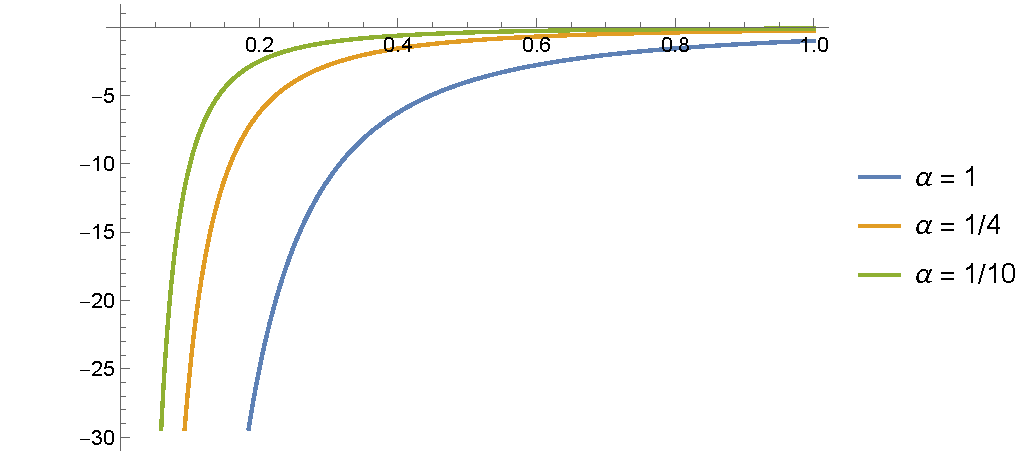
\includegraphics[width=0.8\linewidth]{potential.pdf}
    \caption{The $-\alpha/x^2$ function.}
    \label{fig:potential}
\end{figure}

\vspace{4mm}
\noindent
Let's pretend that we haven't noticed the problem. We're looking for bounded energy states (\textit{i.e. \(E < 0\)}) that are normalized and solutions of the Schrödinger equation:
\begin{align}
    - \frac{\hbar^2}{2m} \frac{d^2\psi}{dx^2} - \frac{a}{x^2}\psi = E \psi
    \label{eq:eigenvalue_boundstate}
\end{align}

where the naive boundary condition are
\begin{align*}
    \lim_{x \to 0} \psi = 0 \quad \text{and} \quad \lim_{x \to +\infty} \psi = 0
\end{align*}

\noindent
Since our intuition leads us to require the wave function to be zero on the negative half-axis and continuous, as well as square-integrable.
\footnote{The latter condition exclude some pathological cases of square integrable functions that does not converge at infinity such $f(x) = x^2 e^{-x^8 \sin^2(x)}$.}

\subsection{The scale invariance symmetry}
Keeping in mind what we have build until now, we want to show the symmetry of our problem on the half-axis, that is the scale invariance and then we want to show what does it imply.

So suppose we found a bound state $\psi(x)$ (\textit{i.e. $E<0$}), that means it satisfies the Equation~\eqref{eq:eigenvalue_boundstate}.

Scaling the variable $x$ by a factor $\beta$, we can easily construct a new solution $\psi_\beta (x) := \psi (\beta x)$ with energy $\beta^2 E$:
\begin{align*}
    H \psi_\beta
     & = - \frac{\hbar^2}{2m} \frac{d^2}{dx^2}\psi_\beta(x) - \frac{a}{x^2} \psi_\beta(x)                                  \\
     & = - \frac{\hbar^2}{2m} \frac{d^2}{dx^2}\psi(\beta x) - \frac{a}{x^2} \psi(\beta x)                                  \\
     & = - \beta^2 \frac{\hbar^2}{2m} \frac{d^2}{d(\beta x)^2} \psi(\beta x) - \beta^2 \frac{a}{(\beta x)^2} \psi(\beta x) \\
     & = - \beta^2 \left(\frac{\hbar^2}{2m} \frac{d^2}{d(\beta x)^2} - \frac{a}{(\beta x)^2}\right) \psi(\beta x) \\
     & = \beta^2 E \, \psi_\beta (x)
\end{align*}
Since $\beta \in \mathbb{R}$ is arbitrary, we can construct an eigenfunction for each negative eigenvalue (remember that we supposed the existence of a bound state). That means that the lowest energy level is $E = -\infty$ (\textit{i.e. it doesn't exist}).

So we can conclude that if a problem is scale invariant, it cannot admit a ground state.\footnote{The absence of the ground state that we've just derived will turn out to be an indication of the inconsistency of the problem we've introduced with Quantum Mechanics, as we will reach a different conclusion in Section~\ref{section:xsqared_halfaxis}.}

\vspace{4mm}
\noindent
What we have learned from the scale invariance is that for every $a$ the $-a/x^2$ potential has no ground state and the allowed energies for bounded states (if they exist) are not quantized, but we can discuss if the value of $a$ has relevance in the existence of a bound state.

First, let's rewrite our problem to make its mathematical aspects clearer: by multiplying Eq.~\eqref{eq:eigenvalue_boundstate} by $2m/\hbar^2$, we obtain:
\footnote{We conventionally use \(\rho\) for bound states and \(k\) for scattering states.}
\begin{align}
    - \frac{d^2\psi}{dx^2} - \frac{\alpha}{x^2}\psi = - \rho^2 \psi, \quad  -\rho^2 := \frac{2mE}{\hbar^2}, \quad \alpha := \frac{2ma}{\hbar^2}.
    \label{eq:eigenvalue_boundstate_alpha}
\end{align}

\subsubsection{Case: \(\alpha < 0\)}
Obviously, since in this situation the potential becomes repulsive, bound states are forbidden.

\subsubsection{Case: \(\alpha < 1/4\)}

To show some properties of this case it's convenient to define $\nu \, (1-\nu) := \alpha$, and then rewrite our Hamiltonian as follow:
\begin{align*}
    H & = - \frac{\hbar^2}{2m} \left(\frac{d^2}{dx^2} + \frac{\alpha}{x^2}\right) \\
      & = - \frac{\hbar^2}{2m} \left( \frac{d}{dx} + \frac{\nu}{x} \right) \left( \frac{d}{dx} - \frac{\nu}{x} \right) = - \frac{\hbar^2}{2m} A B
\end{align*}
Where we defined $A$ and $ B $ respectively as the two differential operators in the parenthesis.

Let show its correctness acting of a test function $f(x)$:
\begin{align*}
    A B f
     & = A \left( \frac{d}{dx} - \frac{\nu}{x} \right) f                                     \\
     & = A \left( f' - \frac{\nu}{x} f \right)                                               \\
     & = \left( \frac{d}{dx} + \frac{\nu}{x} \right) \left( f' - \frac{\nu}{x}f \right)      \\
     & = f'' + \frac{\nu}{x^2} f - \frac{\nu}{x} f' + \frac{\nu}{x} f' - \frac{\nu^2}{x^2} f \\
     & = f'' + \frac{\nu \, (1-\nu)}{x^2} f                                                  \\
     & = \left( \frac{d^2}{dx^2} + \frac{\alpha}{x^2} \right) f .
\end{align*}

\noindent
Before the next step it's useful to notice that $A^\dagger = - B^*$:

\begin{align*}
    \langle f | A g \rangle
     & = \int_{0}^{\infty} f^* \left( \frac{d}{dx} + \frac{\nu}{x} \right) g                                                            \\
     & = f^* g \Big|_0^\infty - \int_{0}^{\infty}  \left[\left( \frac{df}{dx} \right)^* g + \left( \frac{\nu^* f}{x} \right)^* g\right] \\
     & = - \int_{0}^{\infty} \left( \frac{df}{dx} - \frac{\nu^* f}{x} \right)^* g                                                       \\
     & = - \langle B^* f |  g \rangle
\end{align*}

provided that $f$ and $g$ vanish at zero and infinity.

\vspace{4mm}
\noindent
So now we can obtain a formula for the energy of a given state $\psi$ using $A$ and $B$:
\begin{align*}
    E & = \langle \psi | H \psi \rangle             \\
      & = - \frac{\hbar^2}{2m} \langle \psi | A B \psi \rangle         \\
      & = - \frac{\hbar^2}{2m} \langle A^\dagger \psi | B \psi \rangle \\
      & = \frac{\hbar^2}{2m} \langle B^* \psi | B \psi \rangle
\end{align*}
That means if $\nu$ is real, then $B^* = B$, and as a result, $E = (\hbar^2/2m) || B \psi ||^2$, which is strictly greater than zero. Therefore, we have concluded that the realness of $\nu$ precludes the existence of negative energy states (\textit{i.e. no bound states}).\footnote{This result will be shown to be incorrect in Section~\ref{section:xsqared_halfaxis}. The cause of this discrepancy lies in the fact that, with the correct boundary conditions, the boundary term does not vanish.}
This condition, since
\begin{equation*}
    \nu = \frac{1}{2} \pm \sqrt{\frac{1}{4} - \alpha}
\end{equation*}

is equivalent to the condition $\alpha < 1/4$.

\subsubsection{Case: \(\alpha > 1/4\)}

This case imply that $\nu$ is not purely real, so the existence of bound state is not forbidden. Let's look for the bound state trough the Frobenius method, so writing $\psi(x)$ as the following power series
\begin{align*}
    \psi(x) = x^s \sum_{j=0}^{\infty} a_j x^j \quad a_0 \neq 0
\end{align*}

and substituting in the Schrodinger equation \eqref{eq:eigenvalue_boundstate}, we obtain (multiplying by $-1/x^s$)
\begin{align*}
    \sum_{j=0}^{\infty} a_j [(j+s)(j+s-1) + \alpha] x^{j-2} = \rho^2 \sum_{j=0}^{\infty} a_j x^j
\end{align*}
Which, since $a_0 \neq 0$, for the $1/x^2$ term yields $s(s-1)+\alpha = 0$ (\textit{i.e. $s = \nu$}), while fot the $1/x$ term yields $a_1 [(1+s)s + \alpha] = 0$. Using the relation between $\alpha$ and $s$ the equation becomes $a_1 2 s = 0$, but since $s$ is already determined, $a_1 = 0$.

The remaining coefficient are determined by recursion, we can show it changing variable in the left sum: $l + 2 = j$
\begin{align*}
    \sum_{l=0}^{\infty} a_{l+2} [(l+2+s)(l+s+1) + s(1-s)] x^{l} = \rho^2 \sum_{j=0}^{\infty} a_j x^j
\end{align*}

rewriting $(l+2+s)(l+s+1) + s(1-s) $ and equate like powers, so we obtain:
\begin{align*}
    a_{j+2} = \frac{\rho^2}{(2+l)(1+l+2s)} a_j \quad j \in \mathbb{N}
\end{align*}

\noindent
Now remembering that $s$ has two solutions (like $\nu$), from now on called $s_\pm$, $\psi(x)$ will have two solutions too (remember also that we're solving a second order differential equation). Those solutions behave near the origin in the following way
\begin{align*}
    \psi_\pm (x) \approx a_0 x^{s_\pm}, \quad s_\pm = \frac{1}{2} \pm \sqrt{\frac{1}{4} - \alpha}
\end{align*}
That, for $\alpha > 1/4$, means $\psi_\pm (x) \propto \sqrt{x} e^{\pm ig \ln(x)}$ where $g := \sqrt{\alpha-1/4}$.

\vspace{4mm}
\noindent
From the computation of the coefficients $a_j$ turns out that the general solution is the linear combination of the Bessel functions of order $ig$: $A \sqrt{x} K_{ig}(\rho x) + B \sqrt{x} I_{ig}(\rho x)$.~\cite{garfken67:math} The normalization constrain impose $B=0$, so we're left with the solution~\cite{gradshteyn2007}
\begin{align*}
    \psi_\rho(\rho x) = A \sqrt{x} K_{ig}(\rho x), \quad A = \rho \sqrt{\frac{2 \sinh(\pi g)}{\pi g}}
\end{align*}
We know also that the modified Bessel function $K_{ig}$ is real as long as $g$ is real (\textit{i.e. $\alpha>1/4$}), so we can show its functional form in the Fig. \ref{fig:bessel}.

%%% figura bessel
\begin{figure}
    \centering
    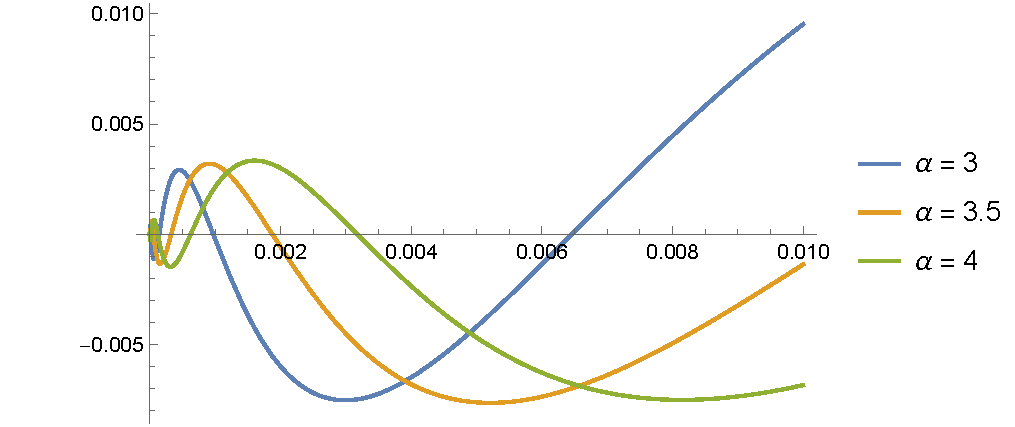
\includegraphics[width=0.8\linewidth]{bessel.pdf}
    \caption{The $\sqrt{x} K_{ig} (\rho x)$ function, $\rho = 1$.} % qua serve caption
    \label{fig:bessel}
\end{figure}

The plot shows the oscillatory behavior of the function near the origin, which is the effect of the sinusoidal dependence on $g \ln(x)$.

It can be shown that the solution has an infinite number of zero crossings, regardless of its energy. Therefore, if the number of zero crossings corresponds to the number of solutions with lower energy, it implies that there's no ground state because it would have $-\infty$ energy, coherent to what we concluded from the scale invariance. \footnote{This observation is consistent with the variational principle.}

\vspace{4mm}
\noindent
Comparing this result to the previous Section~\ref{section:generic_potentials}, in this case, the same behavior occurs as for $s > 2$ (in the old notation), meaning the particle \textit{falls} towards the origin.

\subsection*{Conclusion}
We have showed that the $-a/x^2$ potential has no ground state, no matter the value of $a$, but we have already some differences.
Remembering that $\alpha = 2ma/\hbar^2$, if $\alpha<1/4$, negative energy states (\textit{i.e. bound states}) are not allowed, else if $\alpha > 1/4$, negative energy states are allowed but not quantized (every negative energy is admissible).

\vspace{4mm}
\noindent
It is important to note that the result for $\alpha < 1/4$ will be shown to be incorrect by the end of Section~\ref{section:xsqared_halfaxis}. Even if we don't know it yet, this highlights the consequences of the problem being described by a non self-adjoint Hamiltonian.

\cleardoublepage{}

\chapter{The Method}
%%%%%%%%%%%%%%%%%%%%%%%%%%%%%%%%%%%%%%%%%

\section{The Method of Self-Adjoint Extension}
\label{section:self_adjoint}
This chapter is freely inspired by the work of Bonneau, Faraut and Valent~\cite{Bonneau_2001}.
In physics, self-adjoint operators are
fundamental because they ensure that the associated observables have real
eigenvalues, and real eigenvalues are essential for physical interpretations of
measurements.

Most of our experience and intuition is predicated on the self-adjointness of the operators, and when this fails, the intelligibility of the theory goes with it.

Not all operators in quantum mechanics are self-adjoint by default, it may
depend on the operator itself or its considered domain.\footnote{For example,
    the momentum operator in one dimension is not self-adjoint on its maximum
    domain because its domain is not the entire Hilbert space, \textit{i.e. it's unbounded}.}

The method of self-adjoint extension provides a systematic approach to extend
or restrict the domain of a non-self-adjoint operator to make it self-adjoint.

The process we are about to describe can be summarized as follows: we begin with a symmetric operator $(A,\mathcal{D}(A))$ and gradually extend $\mathcal{D}(A)$ while simultaneously narrowing down $\mathcal{D}({A^\dagger})$ until the two domains become identical. This procedure gives rise to a set of important questions, which were initially tackled by Weyl and subsequently extended by von Neumann and Stone: 

How can one determine if a given operator allows for a self-adjoint extension? 

Is the extension, if it exists, unique? 

How is the self-adjoint domain constructed?


\vspace{4mm}
\noindent
This \textit{Mathematical Tool} chapter aims to answer those questions, but before we can delve into the essence of the method, we need some definitions.

\paragraph{Definition} Let us consider a Hilbert space $\mathcal{H}$. An operator $(A, \mathcal{D}(A))$ defined
on $\mathcal{H}$ is said to be densely defined if the subset $\mathcal{D}(A)$ is dense in
$\mathcal{H}$, meaning that for any $\psi \in \mathcal{H}$, one can find a sequence $\varphi_n$ in
$\mathcal{D}(A)$ that converges in norm to $\psi$.

\paragraph{Definition} An operator $(A, \mathcal{D}(A))$ is said to be closed if there exists a
sequence $\varphi_n$ in $\mathcal{D}(A)$ such that
\[
    \lim_{n \to \infty} \varphi_n = \varphi, \quad \lim_{n \to \infty} A\varphi_n = \psi,
\]
then it follows that $\varphi \in \mathcal{D}(A)$ and $A\varphi = \psi$.

Fortunately all the operators that we use in the rest of the essay are dense and closed, so we shouldn't worry about those conditions.

\paragraph{Definition} The adjoint operator of a (generally unbounded) operator $H$ with a dense
domain $\mathcal{D}(H)$ is defined as follows. The domain
$\mathcal{D}(H^\dagger)$ is the space of functions $\psi$ such that the linear
form
\[
    \varphi \mapsto \langle \psi| H\varphi \rangle
\]
is continuous with respect to the norm of $H$. This implies the existence of
$\psi^\dagger \in H$ such that
\[
    \langle\psi| H\varphi \rangle = \langle\psi^\dagger| \varphi \rangle .
\]
Hence, $H^\dagger\psi = \psi^\dagger$. Notably, the adjoint of any densely
defined operator is closed.

\paragraph{Definition} An operator $(H, \mathcal{D}(H))$ is said to be symmetric if for all $\varphi,
    \psi \in \mathcal{D}(H)$, we have
\[
    \langle H\varphi| \psi \rangle = \langle \varphi| H\psi \rangle.
\]
If $\mathcal{D}(H)$ is dense, this is equivalent to saying that $(H^\dagger,
    \mathcal{D}(H))$ is an extension of $(H, \mathcal{D}(H))$.

\paragraph{Definition} The operator $H$ with dense domain $\mathcal{D}(H)$ is considered self-adjoint
if $\mathcal{D}(H^\dagger) = \mathcal{D}(H)$ and $H^\dagger = H$.

\clearpage

\subsection{The Deficiency Indices}

In this section, we assume that $(A, \mathcal{D}(A))$ is densely defined,
symmetric, and closed, and let $(A^\dagger, \mathcal{D}(A^\dagger))$ be its
adjoint.

We define the deficiency subspaces $\mathcal{N}^+$ and $\mathcal{N}^-$ as
follows:
\[
    \mathcal{N}^+ = \{\psi \in \mathcal{D}(A^\dagger), \quad A^\dagger\psi = z^+\psi, \quad \text{ Im } z^+ > 0\},
\]
\[
    \mathcal{N}^- = \{\psi \in \mathcal{D}(A^\dagger), \quad A^\dagger\psi = z^-\psi, \quad \text{ Im } z^- < 0\},
\]

with respective dimensions $n^+$ and $n^-$. These are referred to as the
deficiency indices of the operator $A$ and will be denoted by the ordered pair
$(n^+, n^-)$.

Importantly, $n^+$ (or $n^-$) is independent of the choice of $z^+$ (or $z^-$)
as long as it lies in the upper (or lower) half-plane. Consequently, one simple
way to determine $(n^+, n^-)$ is to take $z^+ = i\eta$ and $z^- = -i\eta$
with an arbitrary strictly positive constant $\eta$ for dimensional reasons.

\vspace{4mm}
\noindent
The following theorem, by Weyl and von Neumann, is of primary importance.

\subsubsection*{Theorem:}

For an operator $A$ with deficiency indices $(n^+, n^-)$, there are three possibilities:
\begin{enumerate}
    \item If $n^+ = n^- = 0$, then $A$ is self-adjoint (in fact, this is a necessary and
          sufficient condition).
    \item If $n^+ = n^- = n \geq 1$, then $A$ has infinitely many self-adjoint
          extensions, parametrized by a unitary $n \times n$ matrix (\textit{i.e. $n^2$ real parameters}).
    \item If $n^+ \neq n^-$, then $A$ has no self-adjoint extension.
\end{enumerate}

\noindent
The application of this theorem to differential operators requires substantial
work. Even if we start with an operator $P$ that is formally self-adjoint, this
does not guarantee that $P$ is truly self-adjoint because the domains
$\mathcal{D}(P)$ and $\mathcal{D}(P^\dagger)$ will generally be different.

For a given differential operator $P$, three problems need to be solved:
\begin{enumerate}
    \item Find a domain $\mathcal{D}(P)$ for which the formally self-adjoint operator $P$
          is symmetric and closed.
    \item Compute its adjoint $(P^\dagger, \mathcal{D}(P^\dagger))$ and determine the
          deficiency indices of $P^\dagger$.
    \item When they do exist, describe the domains of all the self-adjoint extensions.
\end{enumerate}

\vspace{4mm}
\noindent
In this section, we have briefly described the process to understand the existence, the uniqueness and the dimension of the space of self-adjoint extensions.

\subsection{The Boundary Conditions}

Now we need to provide a method to compute boundary conditions that make our operator $H$ self-adjoint.

For simplicity we assume that the deficiency indices are $n_+ = n_- = 1$, \textit{i.e. $(1,1)$}. Then we expect to find $\phi_+$ and $\phi_-$ as eigenfunction with respect to the two imaginary eigenvalues, \textit{i.e. two generators of the subspaces $ \mathcal{N}_\pm $}.

We also know that the unitary matrix that relates the two one dimensional subspaces $ \mathcal{N}_\pm $ is one-dimensional, \textit{i.e. a complex number of modulus one}. Hence, the self-adjoint extensions depend on one parameter only.

We set $U = \lambda$ with $|\lambda| = 1$, and define $\Phi_\lambda = \phi_+ + \lambda \phi_-$. The prescription for obtaining the boundary conditions is simply to require that:
\begin{align} 
    \label{eq:boundary_condition}
    \langle H \Phi_\lambda | \psi \rangle = \langle \Phi_\lambda | H \psi \rangle
\end{align}

\noindent
All and only the $\psi$ that satisfy this condition are in the domain of the $\lambda$-self-adjoint extension of the operator $H$, \textit{i.e. $(H,\mathcal{D}_\lambda(H))$}.
\cleardoublepage{}

\chapter{Content}
%%%%%%%%%%%%%%%%%%%%%%%%%%%%%%%%%%%%%%%%%

\section{The free particle on the half line}
\label{section:free_halfaxis}
This section, freely inspired by the work of Bonneau, Faraut and Valent~\cite{Bonneau_2001}, is aimed at introducing the concept of self-adjoint extensions of an Hamiltonian operator. 
However, the choice of the free particle on the half-line is not arbitrary, as it represents our original problem where $a = 0$ is imposed. Consequently, we can verify the results obtained from the particle in the potential by considering the scenario where we force $a$ to vanish.

\paragraph*{Note:}
Since this problem is a specific case of a larger one, we know that it inherits its properties, including the important feature of scale invariance, which prohibits the existence of a ground state.\footnote{If we consider some particular boundary conditions, or we don't consider them at all.}

\vspace{4mm}
\noindent
Let's apply the previous analysis to the Hamiltonian operator \(H = -(\hbar^2/2m)d^2/dx^2\).
In this section, we initially approach the problem from a mathematical perspective, leading us to the discovery that there are infinitely many self-adjoint extensions parameterized by \(U(1\)), which corresponds to a phase. Only in the end will be demonstrated that, in this problem, the seemingly straightforward boundary conditions that we might choose intuitively as physicists make already $H$ self-adjoint, differently from what will happen in Section~\ref{section:xsqared_halfaxis}.

\clearpage

\subsection{The Self-adjoint Extensions}
In this section, we apply the previous theorem.

\subsubsection*{The Deficiency Indices}

Let us consider the Hilbert space $\mathcal{H} = \mathcal{L}^2(0,\infty)$
, and to use von Neumann's theorem, we have to determine the functions $\phi_{\pm}(x)$ given by:
\begin{equation} \label{eq:free_H}
    H^\dagger \phi_{\pm}(x) = - \frac{\hbar^2}{2m} \frac{d^2}{dx^2} \phi_{\pm}(x) = \pm \frac{\hbar^2}{2m} ik^2_0 \phi_{\pm}(x), \quad k_0 > 0
\end{equation}

\noindent
An easy integration gives:
\begin{equation*}
    \phi_{\pm} = a_{\pm}e^{k_{\pm}x} + b_{\pm}e^{-k_{\pm}x}, \quad k_{\pm} = \frac{1 \mp i}{\sqrt{2}} k_0 = e^{\mp i \pi/4} k_0
\end{equation*}

\noindent
Then we have to discuss what happens on our interval $[0,\infty)$, the positive semi-axis.
\paragraph{Note:}
For dimensional reasons, we have introduced the constant $k_0$, and, as we preannounced in Section~\ref{section:self_adjoint}, its introduction is compelled by the method.

\vspace{4mm}
\noindent
In the Hilbert space \(\mathcal{H} = \mathcal{L}^2(0, +\infty)\), we have normalized solutions to Eq.~\eqref{eq:free_H} given by:
\begin{align} \label{eq:freepart_eigenfun}
    \phi_{\pm} = b_{\pm}e^{-e^{\mp i \pi/4} k_0 x}, \quad b_\pm = e^{\mp i \pi /4} k_0 (= k_\pm)
\end{align}

\noindent
Since the $a_\pm$ terms grow exponentially, they're not integrable. This leads to deficiency indices \((1, 1)\), resulting in infinitely many self-adjoint extensions parametrized by \(U(1)\), such that $U = e^{i\theta}$ with $\theta \in [0,2\pi]$.
 
\clearpage

\subsubsection*{The Boundary Conditions}

To find the space that makes $H$ self-adjoint, we need to find the $\psi$ that satisfies Eq.~\eqref{eq:boundary_condition}. Defining $\Phi_\theta = \phi_+ + e^{i\theta} \phi_-$, we need the following to vanish:

\begin{align*}
    \langle \Phi_\theta | H \psi \rangle - \langle H \Phi_\theta |  \psi \rangle
     & = \frac{\hbar^2}{2m} \left(\langle \Phi_\theta | - \frac{d^2}{dx^2} \psi \rangle - \langle - \frac{d^2}{dx^2} \Phi_\theta |  \psi \rangle \right)                                                                 \\
     & =  \frac{\hbar^2}{2m} \left(\int_0^\infty -\overline{\Phi_\theta} \psi'' + \int_0^\infty \overline{\Phi_\theta''} \psi \right)                                                                      \\
     & = \frac{\hbar^2}{2m} \left((-\overline{\Phi_\theta} \psi')\Big|_0 + \int_0^\infty \overline{\Phi_\theta'} \psi' + \int_0^\infty \overline{\Phi_\theta''} \psi  \right)                              \\
     & = \frac{\hbar^2}{2m} \left((-\overline{\Phi_\theta} \psi' + \overline{\Phi_\theta'} \psi)\Big|_0 - \int_0^\infty \overline{\Phi_\theta''} \psi + \int_0^\infty \overline{\Phi_\theta''} \psi\right) \\
     & = \frac{\hbar^2}{2m} \left((-\overline{\Phi_\theta} \psi' + \overline{\Phi_\theta'} \psi)\Big|_0\right)
\end{align*}

\noindent
So we need: $\overline{\Phi_\theta}(0) \psi'(0) = \overline{\Phi_\theta'}(0) \psi(0)$ as $x \rightarrow 0$.

If we replace the values of $\Phi_\theta (0)$ and its derivative:
\begin{align*}
    \overline{\phi_+(0) + e^{i\theta} \phi_-(0)} \psi'(0) = \overline{\phi_+'(0) + e^{i\theta} \phi_-'(0)} \psi(0)
\end{align*}

\noindent
Computing the values of $\phi_\pm'$:
\begin{align*}
    \phi_\pm' (x) = -k_\pm b_\pm e^{-k_\pm x} = -k_\pm^2 e^{-k_\pm x}
\end{align*}

\noindent
So, evaluating everything at zero and substituting, the condition becomes:
\begin{align*}
    (\overline{k_+ + e^{i\theta}k_-}) \psi'(0) & = (\overline{-k_+^2 - e^{i\theta} k_-^2} )\psi(0) \\
    (k_- + e^{-i\theta}k_+) \psi'(0)           & = -(k_-^2 + e^{-i\theta} k_+^2 )\psi(0)
\end{align*}
Rearranging the terms
\begin{align*}
    \frac{\psi'(0)}{\psi(0)}
     & = - \frac{k_-^2 + e^{-i\theta} k_+^2}{k_- + e^{-i\theta}k_+}                                                                         \\
     & = - k_0 \frac{e^{i \pi /2} + e^{-i\theta} e^{- i \pi /2}}{e^{i \pi /4} + e^{-i\theta}e^{- i \pi /4}}                                 \\
     & = - k_0 \frac{e^{-i\theta/2}e^{i \pi /2} + e^{-i\theta/2} e^{- i \pi /2}}{e^{-i\theta/2}e^{i \pi /4} + e^{-i\theta/2}e^{- i \pi /4}} \\
     & = - k_0 \frac{\cos(\theta/2 + \pi/2)}{\cos(\theta/2 + \pi/4)}
\end{align*}

\noindent
The term on the right of this equation can assume every real value for $\theta \in [0,2\pi]$.

\clearpage
\noindent
So the final form of the boundary conditions is:

\begin{equation} \label{half_BC}
    \psi(0) = x_0 \psi'(0)  \quad x_0 \in \mathbb{R}
\end{equation}

\noindent
The boundary condition \(\psi'(0) = 0\) corresponds to \({x_0} = \infty\). The most commonly used extension in physics is \({x_0} = 0\), which implies \(\psi(0) = 0\). The latter derives from the infinite potential for $x<0$ and the continuity of the wave function.

\paragraph{Note:}
The ${x_0}$ that characterizes the boundary condition of its corresponding self-adjoint extension is not dimensionless; in fact, it has the dimension of length. Therefore, we have introduced a new parameter, and the dimensional problem of constructing a formula for the eigenvalues is solved. We can say that now that we've our problem provided with boundary conditions that make it self-adjoint, for a generic parameter ${x_0}$ there's no more scale invariance.
\footnote{If we choose ${x_0}=0$ (\textit{i.e. the real physical problem}) the symmetry is still present.}

\subsubsection*{The Dimensional Analysis}
The dimensional parameters of the corresponding quantum mechanical problem, provided with generic boundary conditions, would be:

\begin{align*}
    [\hbar] = E \cdot T, \quad [m] = E \cdot T^2 \cdot L^{-2}, \quad [{x_0}] = L.
\end{align*}

\noindent
So we want to look for three parameters $\alpha$, $\beta$, and $\delta$ that satisfy

\begin{align*}
    E & = \hbar^\alpha m^\beta {x_0}^\delta                                      \\
      & = (E \cdot T)^\alpha (E \cdot T^2 \cdot L^{-2})^\beta (L)^\delta           \\
      & = E^{\alpha + \beta} \cdot T^{\alpha + 2\beta} \cdot L^{-2\beta + \delta}.
\end{align*}

\noindent
So, we are led to an equation for each quantity, \textit{i.e. the system}:

\begin{align}
    \begin{cases}
        E: & 1 = \alpha + \beta   \\
        T: & 0 = \alpha + 2\beta  \\
        L: & 0 = -2\beta + \delta
    \end{cases}
    \quad
    \begin{cases}
        1 = - \beta      \\
        \alpha = -2\beta \\
        \delta = 2\beta
    \end{cases}
    \quad
    \begin{cases}
        \beta = -1 \\
        \alpha = 2 \\
        \delta = -2
    \end{cases}
    \label{eq:free_par_dimensional}
\end{align}

\clearpage

\noindent
This free particle theory for a generic self-adjoint extension has a formula for the eigenvalues proportional to $\hbar^2/m {x_0}^2$. It is important to note that this formula depends on the arbitrary choice of the extension. The physics depends on it, or from a different point of view, the physics can select a particular self-adjoint extension.

\vspace{4mm}
\noindent
Now, let's discuss the energy spectra of a particle confined in the region \(x \geq 0\).

\subsection{The Scattering States}
When the particle energy \(E\) is positive, we can compute the reflection coefficient for this infinitely high barrier (for $x<0$) to compare predictions made by different extensions.

The wave function is:

\[
    \phi(x) = A e^{-ikx} + B e^{ikx}, \quad k^2 := \frac{2mE}{\hbar^2}, \quad k > 0
\]

\noindent
We define the reflection amplitude and reflection probability as follows:

\[
    r(k) = \frac{A}{B},  \quad R(k) = |r(k)|^2
\]

\noindent
Imposing the boundary condition from Eq.~\eqref{half_BC}, we get:

\[
    r(k) = -\frac{1 + i{x_0} k}{1 - i{x_0} k} \implies R = 1 \label{eq:reflection_coefficient}
\]

\begin{figure}
    \centering
    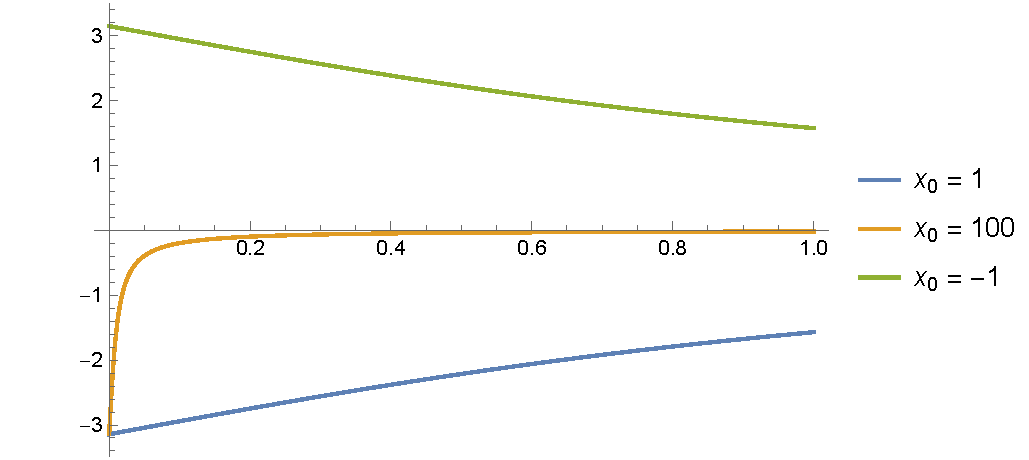
\includegraphics[width=0.8\linewidth]{free_phaseshift.pdf}
    \caption{The $Arg[r(k)]$ function.}
    \label{fig:free_phaseshift}
\end{figure}

\clearpage

\noindent
Remarkably, the physical content (\textit{i.e. \(R = 1\)}) of all the extensions is the same: the wall acts as a perfect reflector. However, the wave function that solves the problem is not independent of the self-adjoint extension, particularly the phase shift of the scattered state (\textit{i.e. $Arg[r(k)]$}), which is plotted in Fig.~\ref{fig:free_phaseshift}.

\vspace{4mm}
\noindent
Here we can introduce an experimental test that checks if the intuition from physics that leads us to impose the ${x_0} = 0$ self-adjoint extension is correct or not.
In fact, as long as an infinitely high wall is experimentally feasible, the dependence from the energy of the scattered wave function phase shift will act as a selector of some self-adjoint extensions. If the experiment says that the phase shift is independent from the energy of the wave function, our physical intuition of the boundary conditions is correct, if not we must take the specific self-adjoint extension that is suggested from the experiment.

\subsection{The Bound States}
With the usual boundary conditions from physics $\phi(0)=0$ (${x_0} = 0$), the presence of a bound state would have been excluded, hence no symmetry breaking. However, considering the generic self-adjoint extension, $\phi(0)$ is no longer restricted to zero, so we can suppose the existence of a bound state.

The wave function solution of the eigenvalue equation $-(\hbar^2/2m)d^2/dx^2 \phi = E \phi$ is:

\[
    \phi(x) = A e^{-\rho x}, \quad - \rho^2 := \frac{2mE}{\hbar^2},  \quad \rho > 0
\]

\noindent
For this wave function, Eq.~\eqref{half_BC} implies \((1 + {x_0}\rho)A = 0\). Since we want to find a non-zero solution: $A \neq 0$, this implies ${x_0}\rho = -1$.

Since $\rho$ should be positive, a bound state with \(\rho = -1/{x_0}\) is only possible when \({x_0} < 0\). So we've found that exist an infinite set of self-adjoint extensions that allows a single bound state, the formula for its energy is as we expected from Eq.~\eqref{eq:free_par_dimensional}.

\vspace{4mm}
\noindent
Now that we are delving into the mathematical aspects of the problem, it's important to note that considering the physical boundary conditions does not result in an anomaly. This is because the physics-motivated boundary conditions already render the Hamiltonian self-adjoint. This specific self-adjoint extension preserves scale invariance, and the theory does not admit bound states.

Conversely, different self-adjoint extensions do not preserve scale invariance. Therefore, in these cases, the presence of a bound state poses no problem.

\clearpage

\noindent
Its energy and normalized wave function are:

\[
    E = - \frac{\hbar^2}{2m{x_0}^2},  \quad {x_0} < 0,  \quad \phi(x) = \sqrt{\frac{2}{|{x_0}|}}e^{-x/|{x_0}|}
\]

\begin{figure}
    \centering
    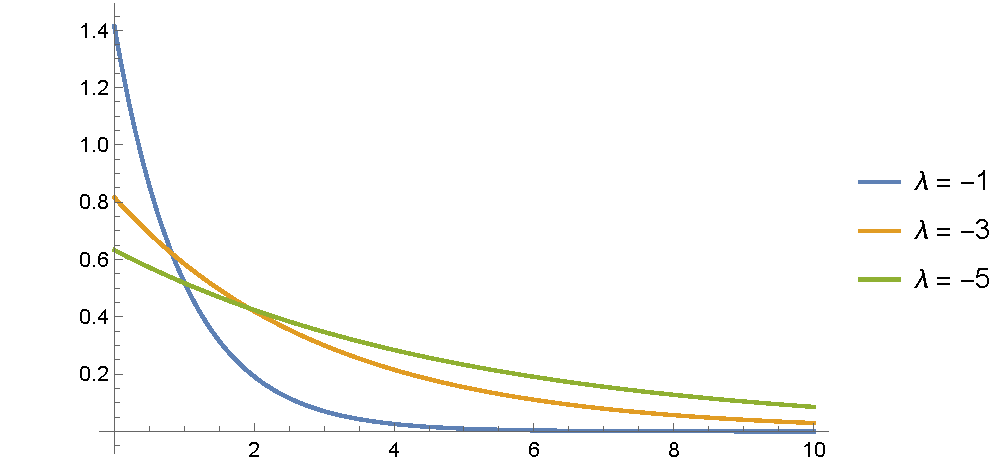
\includegraphics[width=0.8\linewidth]{free_boundstate.pdf}
    \caption{The $\phi(x)$ function.}
    \label{fig:free_boundstate}
\end{figure}

\noindent
Here again we can introduce an experimental test that checks if the intuition from physics that leads us to impose the ${x_0} = 0$ self-adjoint extension is correct or not.
In fact, as long as an infinitely high wall is experimentally feasible, the existence (or non-existence) of this negative energy will act as a selector of some self-adjoint extensions. If the experiment rules out the negative energy state, our intuition could be correct but there are still many possible extensions with \({x_0} \geq 0\). If not, our intuition would have been surely wrong since we've found a unique bound state (plotted in Fig.~\ref{fig:free_boundstate}).

\clearpage

\subsection*{Conclusion}
This chapter provided a simple example of the self-adjoint extension method. Therefore, from a physical perspective, we can employ this method to experimentally verify whether the boundary conditions we have traditionally used accurately describe the examined problem, considering that from a mathematical standpoint, the choice of a self-adjoint extension is arbitrary.

However, if we assume that our physical intuition is correct, the choice would be ${x_0} = 0$, thus preserving scale invariance and its associated consequences: an energy-independent phase shift and the absence of bound states.

\paragraph*{What if our intuition had resulted in an ill-defined problem?}
If, absurdly, our physical intuition had led us to define the boundary condition as $\psi(0) = 1$ (which renders our Hamiltonian operator non-self-adjoint), scale invariance would still be maintained. 
Consequently, based on scale invariance, we would have concluded that there is an energy-independent phase shift and no allowed bound states. 
Nevertheless, since the problem, as posed, doesn't have a self-adjoint Hamiltonian, it would have necessitated a self-adjoint extension.

Mathematically, this would have led us to the same conclusion we have reached in the discussion of this section—namely, a theory that, in general, is not scale-invariant. 
Hence, we would have broken scale invariance symmetry upon quantization, resulting in an anomalous symmetry breaking.

\vspace{4mm}
\noindent
The process we've outlined here is the analogous of what we will discuss in the next section.
\clearpage

\section{The particle in the \texorpdfstring{$1/x^2$}{inverse squared} potential}
\label{section:xsqared_halfaxis}
This Section is freely inspired by the work of Essin and Griffiths~\cite{EssinGriffiths:10.1119/1.2165248}.

In Section~\ref{section:generic_potentials} of this essay, we have demonstrated why the $-a/x^2$ potential differs from other potentials. In the introductory discussion in Section~\ref{section:peculiarities}, we discovered that it cannot possess a ground state because of its scale invariance. By the end of this section, it will become evident that the conclusion we reached is inconsistent with the results of the correct approach to the problem presented in this section.

\vspace{4mm}
\noindent
Now it is time to use the mathematical tool that we've developed in Section~\ref{section:self_adjoint}: \textit{The self-adjoint extension}, to understand all of its subtleties.

\vspace{4mm}
\noindent
The fundamental problem with the $1/x^2$ potential is that the Hamiltonian correlated with our initial \textit{naive} boundary conditions
\begin{equation}
    H =  \frac{\hbar^2}{2m} \left(-\frac{d^2}{dx^2} - \frac{\alpha}{x^2}\right), \quad \lim_{x \to 0} \psi(0) = 0
    \label{eq:naive_BC}
\end{equation}

is not self-adjoint.\footnote{Remember that $\alpha := 2ma/\hbar^2$.}

\vspace{4mm}
\noindent
Let's first show a computation, given $f(x),g(x) \in \mathcal{L}(0,\infty)$:

\begin{align}
    \begin{split}
        \langle f | H g \rangle - \langle H f |  g \rangle
         & = \frac{\hbar^2}{2m} \left(\langle f | (- \frac{d^2}{dx^2} - \frac{\alpha}{x^2}) g \rangle - \langle (- \frac{d^2}{dx^2} - \frac{\alpha}{x^2}) f |  g \rangle\right)                                         \\
         & =  \frac{\hbar^2}{2m} \left(- \int_0^\infty f^* (g''+ \frac{\alpha}{x^2}g) + \int_0^\infty \overline{(f'' + \frac{\alpha}{x^2}f)} g\right)   \\
         & =  \frac{\hbar^2}{2m} \left(- (f^* g')\bigg|_0^\infty + \int_0^\infty f'^* (- g' + \frac{\alpha}{x^2}g) + \int_0^\infty \overline{(f'' + \frac{\alpha}{x^2}f)}\right)                          \\
         & = \frac{\hbar^2}{2m} \left(- (f^* g')\bigg|_0^\infty + (f'^* g)\bigg|_0^\infty - \int_0^\infty f''^* ( g + \frac{\alpha}{x^2}g) + \int_0^\infty \overline{(f'' + \frac{\alpha}{x^2}f)}\right) \\
         & =  \frac{\hbar^2}{2m} \left((- f^* g' + f'^* g)\bigg|_0^\infty - \int_0^\infty \overline{(f''  + \frac{\alpha^*}{x^2}f)}g + \int_0^\infty \overline{(f'' + \frac{\alpha}{x^2}f)}\right) \\
         & = \frac{\hbar^2}{2m} \left((- f^* g' + f'^* g)\bigg|_0^\infty\right)
    \end{split}
    \label{eq:potential_symmetry}
\end{align}
The last identity is true because $\alpha$ is real.

\noindent
We know that for every $f$ and $g$ in $\mathcal{L}(0,\infty)$, at infinity there's no problem since the terms vanish automatically because of the normalization, but the term valued at the origin is more subtle.

We  can easily see that if both $f(x)$ and $g(x)$ respect the boundary condition given by Eq.~\eqref{eq:naive_BC}, then the zero boundary term does not always vanish, since we know that the derivatives can diverge.
In fact, we have shown using the Frobenius method in Section~\ref{section:peculiarities} that the solutions near the origin behave like $x^s$, where $s_\pm = 1/2 \pm \sqrt{1/4 - \alpha}$.

Injecting the founded functional forms in the boundary condition multiplied by $2m/\hbar^2$, we are lead to differentiate for different values of $\alpha$:
\subsubsection*{If $\alpha < 1/4$:} 
Being $f(x) = x^{s_+}$ and $g(x) = x^{s_-}$
\begin{align*}
    (- f^* g' + f'^* g)\bigg|_0
     & = - \overline{x^{s_+}} s_- x^{s_- -1} + \overline{s_+ x^{s_+-1}} x^{s_-} \\
     & = x^{s_+^* + s_- -1}(- s_- + s_+^*)                                      \\
     & = 2 \sqrt{1/4 - \alpha}
\end{align*}

\subsubsection*{If $\alpha > 1/4$:}
 Being $f(x) = x^{s_+}$ and $g(x) = x^{s_+}$
\begin{align*}
    (- f^* g' + f'^* g)\bigg|_0
     & = - \overline{x^{s_+}} s_+ x^{s_+ -1} + \overline{s_+ x^{s_+-1}} x^{s_+} \\
     & = x^{s_+^* + s_+ -1}(- s_+ + s_+^*)                                      \\
     & = 2i \sqrt{\alpha-1/4}
\end{align*}

\vspace{4mm}
\noindent
So we can conclude that unless $\alpha = 1/4$, which is a special limit case we have already encountered and will be discussed separately at the end of this Section and in Section~\ref{section:delta_potential}, a different condition needs to be imposed.

\vspace{4mm}
\noindent
Suppose we require that permissible functions vanish within a finite (albeit extremely small) vicinity of the origin. In such a scenario, the boundary term disappears trivially, and $H$ becomes symmetric within this specific domain. However, if $g(x)$ adheres to this highly constrained domain, $f(x)$ could be any square-integrable function, and the boundary term would still vanish. Consequently, the domain of the adjoint is considerably more extensive than the one of the operator, and, as a result, $H$ does not qualify as self-adjoint.

\subsection{The Self-adjoint Extensions}

Let us apply, recalling the procedure followed in Section~\ref{section:free_halfaxis}, the analysis to the Hamiltonian operator
\begin{align*}
    H = \frac{\hbar^2}{2m} \left(-\frac{d^2}{dx^2} - \frac{\alpha}{x^2}\right),
\end{align*}


on the positive semi-axis, where, anticipating the result, we'll find out that there are infinitely many self-adjoint extensions parametrized by $U(1)$, \textit{i.e. a phase}.

\subsubsection*{The Deficiency Indices}

Let us consider the Hilbert space $\mathcal{H} = \mathcal{L}^2(0, \infty)$, and to use von Neumann's theorem, we have to determine the functions $\phi_{\pm}(x)$ given by
\begin{equation} \label{eq:potential_H}
    H^\dagger \phi_{\pm}(x) = \frac{\hbar^2}{2m} (-\frac{d^2}{dx^2} - \frac{\alpha}{x^2}) \phi_{\pm}(x) = \pm \frac{\hbar^2}{2m} ik^2_0 \phi_{\pm}(x), \quad k_0 > 0
\end{equation}

\noindent
The mathematical literature~\cite{garfken67:math} give us the following result, which is the general solution of the differential equation
\begin{equation*}
    \phi_{\pm} = \sqrt{x}\left(A_\pm H_{ig}^{(1)}(ik_\pm x) + B_\pm H_{ig}^{(2)}(ik_\pm x)\right), \quad k_{\pm} = e^{\mp i \pi/4} k_0
\end{equation*}

where $g := \sqrt{\alpha - 1/4}$, $A_\pm$ and $B_\pm$ are arbitrary constants and $H^{(1)}$, $H^{(2)}$ are Hankel functions.
However, $H_{ig}^{(2)}(x)$ is not in $\mathcal{L}^2(0,\infty)$ (and hence not in $\mathcal{D}({H^\dagger})$) because it diverges exponentially. Thus,
\begin{align*}
    \phi_\pm(x) = A_\pm \sqrt{x} H_{ig}^{(1)}(ik_\pm x)
\end{align*}

where now $A_\pm$ are simply the normalization constants.

\noindent
This leads to deficiency indices \((1, 1)\), resulting in infinitely many self-adjoint extensions parametrized by \(U(1)\), such that $U = \lambda$ with $|\lambda| = 1$ complex, as we anticipated.

\subsubsection*{The Boundary Conditions}

To determine the space in which $H$ is self-adjoint, we need to find the $\psi$ that satisfy Eq.~\eqref{eq:boundary_condition}. By defining $\Phi_\lambda = \phi_+ + \lambda \phi_-$ (notice the dimensionless nature of $\lambda$), we require the following to be zero:
\begin{align*}
    \langle \Phi_\lambda | H \phi \rangle - \langle H \Phi_\lambda |  \phi \rangle
\end{align*}

\noindent
So substituting $\Phi_\lambda$ and $\psi$ in Eq.~\eqref{eq:potential_symmetry}, we obtain the condition:
\begin{align}
    \lim_{x \to 0}\left(\Phi_\lambda^*(x)\frac{d\psi}{dx} - \frac{d\Phi_\lambda^*}{dx}\psi(x)\right) = 0
    \label{eq:potential_bound_explicit}
\end{align}

\noindent
Evidently, we need to understand the behavior of $\phi_\pm$ for small $x$, which requires knowing the behavior of $H_{ig}^{(1)}(x)$. This forces us to split the discussion into different values of $g$.

\subsubsection{Case: \(g \neq 0\)}
Remember that $g \neq 0$ means $\alpha \neq 1/4$.

For a generic non zero value of $g$, the Hankel function $H_{ig}^{(1)}(x)$ behaves near the origin as~\cite{gradshteyn2007}
\begin{equation}
    H_{ig}^{(1)}(ik_\pm x) \approx e^{ig \ln(ik_\pm x/2)}\frac{1 + \coth(\pi g)}{\Gamma(1+ig)} - e^{-ig \ln(ik_\pm x/2)}\frac{\Gamma(1+ig)}{\pi g},
    \label{eq:generig_hankel}
\end{equation}

\noindent
But remembering that $k_\pm = e^{\mp i\pi/4} k_0$,
\begin{equation*}
    \ln(\frac{ik_\pm x}{2}) = \ln(k_0 x)-\ln(2)+ \frac{i l_\pm \pi}{4}
\end{equation*}

where we defined for clarity $l_+ := 1$ and $l_- := 3$.

\noindent
Using this result follow directly that
\begin{equation*}
    e^{ig \ln(ik_\pm x/2)} = e^{ig \ln(k_0 x)}e^{-ig\ln(2)}e^{-g l_\pm \pi/4}
\end{equation*}

\noindent
So we can finally show the functional form of $\phi_\pm$ near the origin:
\begin{align*}
    \phi_+ & \approx \sqrt{x}\left(  D e^{ig \ln(k_0 x)} - F e^{-ig \ln(k_0 x)} \right)                            \\
    \phi_- & \approx \sqrt{x}\left(  D e^{ig \ln(k_0 x)} e^{-\pi g /2} - F e^{-ig \ln(k_0 x)} e^{\pi g /2} \right)
\end{align*}

where we have defined the constants $D$ and $F$ that depend only from $g$ (\textit{i.e. $\alpha$}) as follow
\begin{align*}
    D & := e^{-ig \ln(2)}e^{-\pi g/4}\left( \frac{1 + \coth(\pi g)}{\Gamma(1+ig)}\right) \\
    F & := e^{ig \ln(2)}e^{\pi g/4}\left( \frac{\Gamma(1+ig)}{\pi g}\right)
\end{align*}

\noindent
We have now all the tools to reassemble $\Phi_\lambda$ and compute its derivative, obtaining their behavior near the origin:
\begin{align}
    \Phi_\lambda             & \approx \sqrt{x} \left( G e^{ig \ln(k_0 x)} - J e^{-ig \ln(k_0 x)} \right)                                           \\
    \frac{d\Phi_\lambda}{dx} & \approx \frac{1}{\sqrt{x}} \left( G \frac{1+2ig}{2} e^{ig \ln(k_0 x)} - J \frac{1-2ig}{2} e^{-ig \ln(k_0 x)} \right)
    \label{eq:potential_Phi_deriv}
\end{align}

where we have again defined the new parameters $G$ and $F$ which depend on $\lambda$ and $g$, as

\begin{align*}
    G & := D \, (A_+ +\lambda A_- e^{-\pi g/2}) \\
    J & := F \, (A_+ +\lambda A_- e^{\pi g/2})
\end{align*}

\noindent
Now that we have unraveled the behavior of $\Phi_\lambda$ around the origin, we can come back to the problem of defining the boundary condition of each self-adjoint extension. So using Eq.~\eqref{eq:potential_Phi_deriv} and the general condition reported in Eq.~\eqref{eq:boundary_condition} expressed as in Eq.~\eqref{eq:potential_bound_explicit} (actually we're using its complex conjugate), we obtain the following:
\begin{align}
    \lim_{x \to 0} \sqrt{x}(e^{2ig \ln(x/x_0)} -1 ) \frac{d\psi^*}{dx} - \frac{1}{\sqrt{x}}\left(\frac{1+2ig}{2} e^{2ig \ln(x/x_0)} - \frac{1-2ig}{2} \right) \psi^* = 0
    \label{eq:final_BC}
\end{align}
Where we have introduced a new parameter $x_0$ that is characteristic of the self-adjoint extension; it has incorporated all the parameters defined earlier, so it is $\lambda$ and $\alpha$ dependent. It is defined as followed
\begin{align*}
    x_0 := \frac{1}{k_0} \left( \frac{G}{J} \right)^{i/2g}.
\end{align*}

\subsubsection*{The anomaly in the boundary conditions}

We computed the boundary conditions that render our operator $H$ self-adjoint (\textit{i.e. $\mathcal{D}_\lambda(H) = \mathcal{D}_\lambda(H^\dagger)$}).

The process has necessitated the introduction of a new dimensionless parameter, $\lambda$. However, the calculations have brought about the appearance of $x_0$, which possesses the dimensions of length. This phenomenon breaks the symmetry of our problem, making it no longer scale-invariant.
\footnote{The process that has just happened is an example of dimensional transmutation.}

\vspace{4mm}
\noindent
The thing that has just happened is the anomalous symmetry breaking and we'll talk again about it at the end of the Section.

\subsubsection*{In comparison to the free particle}

We can easily check if the result obtained does accord with the one obtained for the free particle in the half-axis in Section~\ref{section:free_halfaxis}.
In fact taking $\alpha = 0$ (so $g=i/2$) means no potential, and the boundary condition expressed in Eq.~\eqref{eq:final_BC} reduces to:
\begin{align*}
    \lim_{x \to 0} \frac{x_0}{\sqrt{x}} \frac{d\psi^*}{dx} + \frac{1}{\sqrt{x}} \psi^* = 0
\end{align*}

\noindent
Which impose that: the sum of $\psi$ and its derivative approach zero faster than $\sqrt{x}$, and the same condition we've obtained for the free particle discussion:
\begin{align*}
    x_0 \frac{d\psi}{dx}(0) + \psi(0) = 0.
\end{align*}

\subsubsection{Case: \(g = 0\)}
Remember that $g = 0$ means $\alpha = 1/4$.

In this situation the behavior near the origin of the Hankel function we used, Eq.~\eqref{eq:generig_hankel}, is no more correct, we need to replace it by~\cite{gradshteyn2007}

\begin{align}
    H_0^{(1)}(ik_\pm x) \approx 1 - \frac{l_\pm}{2} + \frac{2i}{\pi} \ln\left(\frac{\gamma k_0 x}{2}\right)\
    \label{eq:hankel_g0}
\end{align}

where $\gamma$ is defined as $e^C$ where $C$ is the Euler's constant.

\noindent
Hence, we can express the elements of the deficiency spaces as:

\begin{align*}
    \phi_+ & \approx A_+ \sqrt{x} \left(+\frac{1}{2}+ \frac{2i}{\pi} \ln \left( \frac{\gamma k_0 x}{2} \right)  \right) \\
    \phi_- & \approx A_- \sqrt{x} \left(-\frac{1}{2}+ \frac{2i}{\pi} \ln \left( \frac{\gamma k_0 x}{2} \right)  \right)
\end{align*}

\noindent
So now we have everything to construct $\Phi_\lambda$ and its derivative, they turn out to be

\begin{align*}
    \Phi_\lambda             & \approx \sqrt{x} \left(G + J \ln\left(\frac{\gamma k_0 x}{2}\right)\right)                 \\
    \frac{d\Phi_\lambda}{dx} & \approx \frac{1}{2\sqrt{x}} \left(G + 2J + J \ln\left(\frac{\gamma k_0 x}{2}\right)\right)
\end{align*}

\noindent
We again have defined the variables $G$ and $J$ that are dependent from the self-adjoint extension as follow:
\begin{align*}
    G & := \frac{1}{2} (A_+ - \lambda A_-)    \\
    J & := \frac{2i}{\pi} (A_+ + \lambda A_-)
\end{align*}

\noindent
So the last thing to do is to inject those terms in Eq.~\eqref{eq:potential_bound_explicit}, to find the constrain that defines the domain $\mathcal{D}_\lambda(H)$, where $\psi$ lives, that makes $H$ self-adjoint. The boundary condition turns out to be

\begin{align}
    \lim_{x \to 0} \sqrt{x} \ln\left(\frac{x}{x_0}\right) \frac{d\psi}{dx} - \frac{1}{\sqrt{x}}\left(1+\frac{1}{2} \ln\left(\frac{x}{x_0}\right) \right) \psi =0
    \label{eq:final_BC_g0}
\end{align}

where this time we have defined the dimensional parameter that characterizes the self-adjoint extension as follow
\begin{align*}
    x_0 := \frac{2}{\gamma k_0} e^{-G/J}
\end{align*}

\subsection*{The anomaly in the boundary condition}

As we've briefly mentioned earlier for the case $g \neq 0$, we can say that the process that lead us from the non self-adjoint Hamiltonian operator (because of its boundary conditions) to the family of the self-adjoint ones, introduced a new parameter in the theory.
This parameter, \textit{i.e. $x_0$}, is not dimensionless, indeed has the dimension of a length; it shows up in the new boundary conditions of the Hamiltonian,\textit{i.e. Eq.~\eqref{eq:final_BC} if $g\neq 0$ and Eq.~\eqref{eq:final_BC_g0} if $g=0$ ($\alpha=1/4$)}. So if we try to newly prove the scale invariance of the problem, since the boundary conditions are now not scale invariant, we'll surely fail.

\vspace{4mm}
\noindent
What happened, in physics, is called \textit{anomalous symmetry breaking}, that is the breaking of a symmetry upon quantization.
  
\clearpage

\subsection{The Bound States}

So far, we've computed a continuous set of boundary conditions that define $\mathcal{D}_\lambda(H)$ such that $(H,\mathcal{D}_\lambda(H))$ is self-adjoint, but the selection of a specific extension, or in other words, a particular value for $x_0$, is arbitrary. Consequently, this implies the existence of an entire $U(1)$ one-parameter family of distinct physical theories associated with the $1/x^2$ potential.
This fact raises the question: 

Do these theories yield reasonable bound state spectra?

\vspace{4mm}
\noindent
We know from Section~\ref{section:peculiarities} that if our problem admits negative energy states that are normalizable, \textit{i.e. bound states}, they should assume the following functional form
\begin{align*}
    \psi_\rho(\rho x) = A \sqrt{x} K_{ig}(\rho x), \quad A = \rho \sqrt{\frac{2 \sinh(\pi g)}{\pi g}}
\end{align*}

where $\rho^2 := - 2mE/\hbar^2$.

\noindent
Remembering that $K_{ig}$ is the modified Bessel function and knowing its relation with $H_{ig}^{(1)}$, the Hankel function:
\begin{align*}
    \psi_\rho(\rho x) = A \frac{i\pi}{2} \sqrt{x} H_{ig}(i \rho x), \quad A = \rho \sqrt{\frac{2 \sinh(\pi g)}{\pi g}}
\end{align*}

\noindent
It's now normal to ask if for some self-adjoint extension, the presented bound state satisfy the boundary conditions, \textit{i.e. it is in the self-adjoint domain of $H$}.

\vspace{4mm}
\noindent
To answer we're newly forced to split the discussion for different values of $g$.

\subsubsection{Case: \(g = 0\)}

Since the condition at infinity il already satisfied, we need to expand our function and its derivative in the neighborhood of the origin, from Eq.~\eqref{eq:hankel_g0} 
\begin{align*}
    \psi_\rho &\approx - A \sqrt{x} \ln{ \left( \frac{\gamma \rho x}{2} \right) } \\
    \frac{d\psi_\rho}{dx} &\approx -A \frac{1}{\sqrt{x}} \left(1+\frac{1}{2}\ln{ \left( \frac{\gamma \rho x}{2} \right) }\right)
\end{align*}

\clearpage

\noindent
Imposing the boundary condition we've founded earlier: Eq.~\eqref{eq:final_BC_g0}, we obtain
\begin{align*}
    \lim_{x \to 0} A \ln(\frac{\gamma \rho x_0}{2}) = 0
\end{align*}
So the only solution is satisfied by $\gamma \rho x_0/2 = 1$, \textit{i.e. $\rho = 2/\gamma x_0$}.

\vspace{4mm}
\noindent
What we've found is that for each self-adjoint extension there's a unique bound state, and its energy is dependent from the choice of the self-adjoint extension, so it cannot be calculated if we don't know what self-adjoint extension is the \textit{correct} one that describes our physical problem. 

\vspace{4mm}
\noindent
Mathematically, the choice of a particular extension is arbitrary. However, in reality, our system is described by only one of these extensions. Thus, only a physical experiment, such as measuring the energy of the bound state, can determine the specific self-adjoint extension that describes it.
\footnote{In fact, in some other self-adjoint extension problems that describe physical scenarios, we can eliminate certain self-adjoint extensions that do not align with the physical symmetries that the real problem should adhere to.}

\subsubsection{Case: \(g \neq 0\)}

Now, again we have to impose the self-adjoint boundary conditions on the wave function we know posses negative energy and see if some of them survives.

Knowing the behavior of $K_{ig}$ and its derivative near the origin~\cite{garfken67:math}, reported as follow
\begin{align*}
    \psi_\rho             & \approx B \sqrt{x} \sin{\theta}                                                     \\
    \frac{d\psi_\rho}{dx} & \approx B \frac{1}{\sqrt{x}} \left(\frac{1}{2} \sin{\theta} + g \cos(\theta)\right)
\end{align*}

where we have defined the parameter $B$ and the function $\theta(x)$ as
\begin{align*}
    B         & := -A\sqrt{\frac{\pi}{g \sinh(\pi g)}}      \\
    \theta(x) & := g \ln{\left(\frac{\rho x}{2}\right)} - Arg[\Gamma(1+ig)]
\end{align*}

\clearpage

\noindent
Using now the boundary condition we've founded earlier: Eq.~\eqref{eq:final_BC}, we obtain:

\noindent
If $g$ is real, \textit{i.e. $\alpha > 1/4$}
\begin{align*}
    \rho = \frac{2}{x_0} \, e^{ \frac{Arg \left[\Gamma(1+ig)\right] - n \pi}{g}}, \quad n \in \mathbb{Z}
\end{align*}

that means an infinite set of unbounded discrete eigenvalues, \textit{i.e. no ground state}.

\noindent
If $g$ is imaginary, \textit{i.e. $\alpha < 1/4$}
\begin{align*}
    \rho = \frac{2}{x_0}
\end{align*}

that means an unique bound state for each self-adjoint extension.

\vspace{4mm}
\noindent
The correctness of this result suggest us that when we showed that $\alpha < 1/4$ implies that no negative energy is allowed, in Section~\ref{section:peculiarities}, we've missed something, or more precisely, the problem we considered was described by a non self-adjoint Hamiltonian.

\subsection*{The anomaly in the bound states}

We have already discussed the anomaly that became evident when we identified the appropriate boundary conditions to make $H$ self-adjoint. Since scale invariance is broken, bound states are no longer forbidden; in fact, we have derived a reasonable expression for the spectrum.

\vspace{4mm}
\noindent
As mentioned earlier, the energies obtained depend on $x_0$, making the spectrum measurement the sole method to determine the specific self-adjoint extension that describes our physical problem.

\clearpage

\section{Conclusions}
\label{section:conclusion}
The $1/x^2$ potential with the naive boundary condition: $\psi(x) \to 0$ for $x \to 0$, poses clear challenges. It leads to an infinite and uncountable number of bound states for negative energies, unbounded in absolute value.

\vspace{4mm}
\noindent
Alternatively, one could propose that some potentials in Quantum Mechanics are simply forbidden or nonexistent in the natural world, but I do not agree. There is experimental evidence indicating the existence of physical systems represented, at least approximately, by the $1/x^2$ potential or its three-dimensional analog. A prime example is the interaction of an electron with a stationary electric dipole, such as an electron interacting with a polar molecule. In this case, the potential is $-e p \cos(\theta)/r^2$, and the radial part of the Schrödinger equation aligns mathematically with our discussion. Furthermore, the critical parameter $\alpha = 1/4$ holds significance in the study of this system, as it is associated with the minimum value for the dipole moment or the minimum moment required to bind a charged particle to an extended electric dipole.

\vspace{4mm}
\noindent
In conclusion, the discussion presented in this essay might appear somewhat reminiscent of non-ordinary quantum mechanics. However, this resemblance is likely due to the fact that introductory quantum mechanics courses often teach that certain mathematical intricacies are the domain of mathematicians. This is not always the case, which is why I believe a rigorous mathematical approach to physics should be as fundamental as the teaching of intuition.
\cleardoublepage{}

\chapter{Analogy from the literature} %%%%%%%%%%%%%%%%%%%%%%%%%%%%%%%%%%%%%%%%%

\section{The two-dimensional \texorpdfstring{$\delta$}{Delta}-potential}
\label{section:delta_potential}
The literature on anomalies in quantum mechanics often focuses on two particular situations: the $1/x^2$ potential and the 2-dimensional $\delta$ potential. In this section, we aim to demonstrate that these two problems share some common peculiarities, particularly their scale invariance, which leads to similar discussions.

\vspace{4mm}
\noindent
The Hamiltonian for this problem is: 
\begin{align*}
    H = - \frac{\partial^2}{\partial x^2} - \frac{\partial^2}{\partial y^2} - \delta(x) \delta(y)
\end{align*}

\subsubsection*{The Scale Invariance Symmetry}

Just as with the other potential, let's assume we've found a bound state $\psi(x,y)$ (\textit{i.e. $E < 0$}), which satisfies the equation:
\begin{align*}
    \left(- \frac{\partial^2}{\partial x^2} - \frac{\partial^2}{\partial y^2} - \delta(x) \delta(y)\right)\psi(x,y) = E\psi(x,y)
\end{align*}

\clearpage

\noindent
If we scale the variables $x$ and $y$ at the same time by a factor of $\beta$, we can easily construct a new solution, $\psi_\beta(x,y) := \psi(\beta x, \beta y)$, with energy $\beta^2 E$:
\begin{align*}
     H \psi_\beta (x,y)
     & = - \frac{\partial^2}{\partial x^2}\psi_\beta(x,y) - \frac{\partial^2}{\partial y^2}\psi_\beta(x,y) - \delta(x) \delta(y)\psi_\beta(x,y) \\
     & = - \frac{\partial^2}{\partial x^2}\psi(\beta x, \beta y) - \frac{\partial^2}{\partial y^2}\psi(\beta x, \beta y) - \delta(x) \delta(y)\psi(\beta x, \beta y) \\
     & = - \beta^2 \frac{\partial^2}{\partial (\beta x)^2}\psi(\beta x, \beta y) - \beta^2 \frac{\partial^2}{\partial (\beta y)^2}\psi(\beta x, \beta y) - \beta^2 \delta(\beta x) \delta(\beta y)\psi(\beta x, \beta y) \\
     & = - \beta^2 \left(\frac{\partial^2}{\partial (\beta x)^2} - \frac{\partial^2}{\partial (\beta y)^2} -  \delta(\beta x) \delta(\beta y)\right)\psi(\beta x, \beta y) \\
     & = \beta^2 E \, \psi_\beta (x)
\end{align*}
Because the transformation law of the $\delta$-function produces a $\beta$ factor for each dimension in the change of variable.

This computation confirms the scale invariance of the problem.

\subsubsection*{The Connection}

Now, we want to demonstrate that the $\delta$ potential problem can be viewed as a particular case of the $-\alpha/x^2$ potential problem.~\cite{Araujo_10.1119/1.1624111}

\vspace{4mm}
\noindent
Examine the radial component of the Hamiltonian operator for a free particle in the plane with the origin excluded:

\begin{equation*}
    H = - \frac{1}{r} \frac{d}{dr} \left( r \frac{d}{dr} \right)
\end{equation*}

\noindent
By using the unitary transformation parametrized by $s$:

\begin{align*}
    U_s: \mathcal{L}^2([0, \infty); r^{-2s} dr) & \to \mathcal{L}^2([0, \infty); dr) \\
    (Uf)(r)                                   & = r^s f(r)
\end{align*}

\noindent
The action of the operator becomes:

\begin{align*}
    - \frac{1}{r} \frac{d}{dr} \left(r \frac{d}{dr} \right) r^s f
     & = \left( \frac{d^2}{dr^2} + \frac{1}{r} \frac{d}{dr} \right) r^s f \\
     & =  r^s \left( \frac{s(s-1)}{r^2} f + \frac{2s}{r} f' + f'' \right) +  r^s \left( \frac{1}{r} f' + \frac{s}{r^2} f \right) \\
     & = r^s \left(  \frac{1}{r^2} s^2 f + \frac{1}{r} (2s+1) f' + f''  \right)
\end{align*}

\noindent
To remove the first derivative term and obtain what we want, we set $s = -1/2$. 

Hence our specific operator is

\begin{align*}
    U_{-1/2}: \mathcal{L}^2([0, \infty); r dr) & \to \mathcal{L}^2([0, \infty); dr) \\
    (Uf)(r)                                   & = \frac{1}{\sqrt{r}} f(r)
\end{align*}

\noindent
The overall factor $r^{-1/2}$ is eliminated by the action of $U_{-1/2}^\dagger$, so the action of the Hamiltonian becomes:

\begin{equation*}
    H' = U_{-1/2}^\dagger \, H \, U_{-1/2} = - \frac{d^2}{dr^2} - \frac{1}{4r^2}
\end{equation*}

\noindent
The problem of the $\delta$ potential is revealed to be a specific self-adjoint extension of the free particle in the plane with the origin removed~\cite{Jackiw:216395}. Therefore, for states with circular symmetry, implying the angular wave function is in its ground state, the two-dimensional $\delta$ function problem is mathematically equivalent to the $-\alpha/x^2$ potential, where $\alpha = 1/4$.
\cleardoublepage{}

%%% REFERENCES %%%

\defbibheading{bibliography}[\bibname]{
  \chapter*{References}
  \addcontentsline{toc}{chapter}{References}
  \markboth{\textsc{References}}{}
}

\printbibheading{}
\newrefcontext{myarticles}
\printbibliography[heading=subbibliography,resetnumbers,category=MyArticles,title={Articles covering the presented results}]
\newrefcontext{books}
\printbibliography[heading=subbibliography,resetnumbers,type=book,title={Books}]
\newrefcontext{nonbooks}
\printbibliography[heading=subbibliography,resetnumbers,nottype=book,notcategory=MyArticles,title={Articles}]

\newpage
\pagestyle{empty}
\mbox{}
\clearpage

\end{document}















